\section{Lab: mmap}

\subsection{实验目的}
本实验旨在熟悉进程内存地址的映射机制。mmap 和 munmap 系统调用允许 UNIX 程序对其地址空间进行详细控制。它们可用于在进程之间共享内存,将文件映射到进程地址空间,并作为用户级页面错误方案的一部分。本实验将向 xv6 添加 mmap 和 munmap,重点关注内存映射文件。

\subsection{实验步骤}

\begin{enumerate}
    \item 按照前文的方法,注册两个系统调用sys\_mmap 和sys\_munmap。
    \item 在proc.h文件中添加vma结构体,并把它添加到proc结构体中。vma 结构体表示进程的一个虚拟内存区域。虚拟内存区域用于映射进程的虚拟地址空间到实际物理内存或文件,允许进程访问所需的资源。结构体内的各个字段记录了虚拟内存区域的具体信息,包括起始地址、长度、关联的文件、保护和标志属性等。
          \begin{lstlisting}[language=c,title=vma结构体]
    // 虚拟内存区域(Virtual Memory Area, VMA)结构体
    struct vma {
        int valid;          // 标志此VMA是否有效(1表示有效,0表示无效)
        uint64 addr;        // VMA的起始地址(虚拟地址)
        int len;            // VMA的长度(以字节为单位)
        struct file *f;     // 指向与此VMA关联的文件的指针
        int prot;           // VMA的保护标志(如可读、可写、可执行)
        int flags;          // VMA的标志(如共享、私有映射)
        int fd;             // 文件描述符,用于标识与此VMA关联的文件
        int offset;         // VMA在文件中的偏移量
    };                
    \end{lstlisting}
          \begin{lstlisting}[language=c,title=对proc结构体的修改]
    #define VMASIZE 16
    struct proc
    {
      ...
      struct vma vma[VMASIZE];
    };
    \end{lstlisting}
    \item 修改trap.c文件中的usertrap 函数,添加对缺页的处理。
          \begin{lstlisting}[language=c,title=对usertrap函数的修改]
    void usertrap(void)
    {
        int which_dev = 0;
    
        ...

        else if (r_scause() == 13 || r_scause() == 15)
        {
            // 页面错误(Page Fault)
        
            // 获取发生页面错误的虚拟地址。
            uint64 va = r_stval();
        
            // 检查页面错误的地址是否在有效范围内,如果超出范围,标记进程为 killed。
            if (va >= p->sz || va > MAXVA || PGROUNDUP(va) == PGROUNDDOWN(p->trapframe->sp))
                p->killed = 1;
        
            struct vma *vma = 0;
            // 遍历进程的虚拟内存区域 (VMA),找到与页面错误地址匹配的 VMA。
            for (int i = 0; i < VMASIZE; i++)
            {
                if (p->vma[i].valid && va >= p->vma[i].addr && va < p->vma[i].addr + p->vma[i].len)
                {
                    vma = &p->vma[i];
                    break;
                }
            }
        
            if (vma)
            {
                // 将页面地址向下取整,以页大小为单位对齐。
                va = PGROUNDDOWN(va);
                uint64 offset = va - vma->addr; // 计算偏移量。
                uint64 mem = (uint64)kalloc();  // 分配一页物理内存。
                if (mem == 0)
                {
                    // 如果内存分配失败,标记进程为 killed。
                    p->killed = 1;
                }
                else
                {
                    memset((void *)mem, 0, PGSIZE); // 将分配的内存清零。
                    ilock(vma->f->ip);              // 锁定文件以防止其他进程访问。
                    readi(vma->f->ip, 0, mem, offset, PGSIZE); // 从文件中读取数据到内存中。
                    iunlock(vma->f->ip);            // 解锁文件。
            
                    // 设置页表条目的权限标志。
                    int flag = PTE_U;
                    if (vma->prot & PROT_READ)
                        flag |= PTE_R;
                    if (vma->prot & PROT_WRITE)
                        flag |= PTE_W;
                    if (vma->prot & PROT_EXEC)
                        flag |= PTE_X;
            
                    // 将虚拟地址映射到物理内存。
                    if (mappages(p->pagetable, va, PGSIZE, mem, flag) != 0)
                    {
                        // 如果映射失败,释放分配的内存并标记进程为 killed。
                        kfree((void *)mem);
                        p->killed = 1;
                    }
                }
            }
        }
        ...
    
        usertrapret(); // 从内核模式返回到用户模式,恢复进程执行。
    }    
    \end{lstlisting}
    \item 在sysfile.c文件中添加sys\_mmap和sys\_munmap系统调用的实现。
          \begin{lstlisting}[language=c,title=sys\_mmap的实现]
    uint64 sys_mmap(void)
    {
        struct file *f;       // 文件指针,指向要映射的文件
        int prot, flags, fd, offset, len;
        uint64 addr;
    
        // 从系统调用的参数中获取地址、长度、保护标志、映射标志、文件描述符和偏移量
        // 如果获取参数失败,则返回-1表示错误
        if (argaddr(0, &addr) || argint(1, &len) || argint(2, &prot) ||
            argint(3, &flags) || argfd(4, &fd, &f) || argint(5, &offset))
            return -1;
    
        // 如果文件不可写,并且请求了写权限并且映射类型是共享的,则返回-1
        if (!(f->writable) && (prot & PROT_WRITE) && flags == MAP_SHARED)
            return -1;
    
        struct proc *p = myproc();  // 获取当前进程的指针
        len = PGROUNDUP(len);       // 将长度向上对齐到页面大小
        if (p->sz > MAXVA - len)    // 如果映射超出了虚拟地址空间的最大值,则返回-1
            return -1;
    
        // 查找进程中未使用的虚拟内存区域
        for (int i = 0; i < VMASIZE; i++)
        {
            if (p->vma[i].valid == 0)  // 找到一个空闲的虚拟内存区域
            {
                // 初始化虚拟内存区域的各个属性
                p->vma[i].valid = 1;
                p->vma[i].addr = p->sz;  // 设置映射的起始地址
                p->vma[i].len = len;     // 设置映射的长度
                p->vma[i].f = f;         // 映射的文件
                p->vma[i].prot = prot;   // 保护标志
                p->vma[i].flags = flags; // 映射标志
                p->vma[i].offset = offset; // 文件偏移量
        
                filedup(f);  // 增加文件的引用计数
                p->sz += len;  // 增加进程的虚拟内存大小
        
                return p->vma[i].addr;  // 返回映射的起始地址
            }
        }
        return -1;  // 如果没有可用的虚拟内存区域,则返回-1
    }
                
    \end{lstlisting}
          \begin{lstlisting}[language=c,title=sys\_munmap的实现]
    uint64 sys_munmap(void)
    {
        uint64 addr;
        int len;
    
        // 从系统调用的参数中获取地址和长度
        // 如果获取参数失败,则返回-1表示错误
        if (argaddr(0, &addr) || argint(1, &len))
        return -1;
    
        addr = PGROUNDDOWN(addr); // 将地址向下对齐到页面大小
        len = PGROUNDUP(len);     // 将长度向上对齐到页面大小
    
        struct proc *p = myproc();  // 获取当前进程的指针
        struct vma *vma = 0;
    
        // 查找包含指定地址的虚拟内存区域
        for (int i = 0; i < VMASIZE; i++)
        {
            if (addr >= p->vma[i].addr && addr < p->vma[i].addr + p->vma[i].len)
            {
                vma = &p->vma[i];  // 找到对应的虚拟内存区域
                break;
            }
        }
    
        if (vma == 0)
            return 0;  // 如果未找到对应的虚拟内存区域,则返回0
    
        if (vma->addr == addr)  // 如果地址匹配
        {
            vma->addr += len;    // 更新虚拟内存区域的起始地址
            vma->len -= len;     // 更新虚拟内存区域的长度
        
            // 如果映射类型是共享的,将内存内容写回文件
            if (vma->flags & MAP_SHARED)
                filewrite(vma->f, addr, len);
        
            // 解除映射的内存页
            uvmunmap(p->pagetable, addr, len / PGSIZE, 1);
        
            if (vma->len == 0)  // 如果虚拟内存区域的长度为0
            {
                fileclose(vma->f);  // 关闭与该区域关联的文件
                vma->valid = 0;     // 将虚拟内存区域标记为无效
            }
        }
        return 0;  // 返回0表示成功
    }
                
    \end{lstlisting}
    \item 将vm.c文件中nvmcopy 和uvmunmap 函数的if((*pte \& PTE\_V) == 0) 条件后的panic改为continue。将 panic 改为 continue 后,当检测到无效页面时,程序不会崩溃,而是跳过这个页面,继续处理后续的页面。
    \item 在proc.c文件中修改fork函数,使之可以把父进程的内存映射也添加给子进程。
          \begin{lstlisting}[language=c,title=对fork函数的修改]
    int fork(void)
    {
        int i, pid;
        struct proc *np;         // np指向新创建的子进程结构体
        struct proc *p = myproc(); // p指向当前进程,即父进程
    
        ...
    
        // 复制父进程的虚拟内存区域(VMA)到子进程
        for (int i = 0; i < VMASIZE; i++)
        {
            if (p->vma[i].valid)  // 如果父进程的VMA有效
            {
                memmove(&(np->vma[i]), &(p->vma[i]), sizeof(p->vma[i])); // 复制VMA
                filedup(p->vma[i].f);  // 增加文件的引用计数
            }
        }
        release(&np->lock); // 释放子进程的锁
    
        return pid; // 返回子进程的PID给父进程
    }
                
    \end{lstlisting}
    \item 在proc.h文件中修改exit函数,添加接触映射的功能。
          \begin{lstlisting}[language=c,title=对exit函数的修改]
    void exit(int status)
    {
        ...
    
        // 处理进程的虚拟内存区域(VMA)
        for (int i = 0; i < VMASIZE; i++)
        {
            if (p->vma[i].valid) // 如果虚拟内存区域有效
            {
                // 如果内存映射是共享的,将内存写回文件
                if (p->vma[i].flags & MAP_SHARED)
                filewrite(p->vma[i].f, p->vma[i].addr, p->vma[i].len);
                
                // 关闭与虚拟内存区域相关联的文件
                fileclose(p->vma[i].f);
        
                // 解除映射的内存页
                uvmunmap(p->pagetable, p->vma[i].addr, p->vma[i].len / PGSIZE, 1);
        
                p->vma[i].valid = 0; // 将VMA标记为无效
            }
        }
    
        ...
    }   
                
    \end{lstlisting}
\end{enumerate}

\subsection{评测结果}
利用脚本./grade-lab-mmap评测,得到结果如图\ref{fig:mmap}。
\begin{figure}[h]
    \centering
    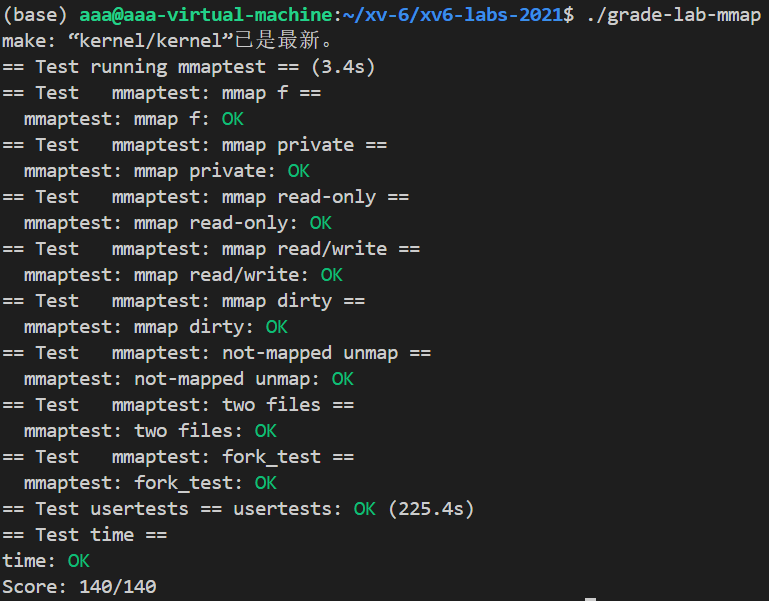
\includegraphics[width=\linewidth]{pics/mmap评测结果.png}
    \caption{mmap评测结果}
    \label{fig:mmap}
\end{figure}
\subsection{实验小结}
在本次实验中,我成功地在 xv6 操作系统中实现了 mmap 和 munmap 系统调用。通过该实验,我深入理解了内存映射的基本概念以及其在操作系统中的应用。

具体来说,我通过 sys\_mmap 系统调用实现了将文件映射到进程的虚拟内存地址空间的功能,使得进程可以直接通过内存访问文件内容,而无需频繁的文件 I/O 操作。这不仅提升了文件访问的效率,还为进程间共享内存提供了基础。

总体而言,本实验使我掌握了内存映射的核心机制,并在 xv6 中实现了这一功能,进一步加深了对操作系统内存管理的理解。这些知识不仅对理解现代操作系统的内存管理至关重要,也为后续的系统开发和优化提供了实践经验。
